 \let\thefootnote\relax\footnotetext{
 Aquest document està baix llicència \href{http://creativecommons.org/licenses/by-sa/3.0/}{Creative Commons Atributive Share-Alike 3.0}
 per tant es pot compartir, modificar i distribuir, però citant els autors originals i sense modificar la llicència.
 De la mateixa manera el codi font està baix llicència GNU GPL v3 per part dels dos autors.\bigskip}
\let\thefootnote\relax\footnotetext{El document en versió digital i el codi font el trobareu a \\ \url{https://github.com/bmiro/raiden}\bigskip}
\let\thefootnote\relax\footnotetext{Aquest document i tota la part de la practica que s'ha pogut ha estat desenvolupat emprant programari lliure:}
\let\thefootnote\relax\footnotetext{\href{http://www.tug.org/applications/pdftex/}{\LaTeX} i \href{http://www.tug.org/applications/pdftex/}{Kile} per el text,
\href{http://www.inkscape.org/}{Inkscape} pels diagrames,
\href{http://kate-editor.org/}{Kate} i \href{http://vim.org/}{Vim} per l'edició del codi font.
\href{http://git-scm.com/}{Git} com a sistema de control de versions.
}

\let\thefootnote\relax\footnotetext{
\begin{center}
\begin{tabular}{cc}

\includegraphics[height=35pt,keepaspectratio=true]{diagrames/by-sa.png}
 & 
\includegraphics[height=35pt,keepaspectratio=true]{diagrames/gnu.png}
\end{tabular}
\end{center}
\begin{center}
\begin{tabular}{cccccc}
 
\includegraphics[height=35pt,keepaspectratio=true]{diagrames/latex.png}
 & 
\includegraphics[height=35pt,keepaspectratio=true]{diagrames/kile.png}
 & 
\includegraphics[height=35pt,keepaspectratio=true]{diagrames/inkscape.png}
 & 
\includegraphics[height=35pt,keepaspectratio=true]{diagrames/kde.png}
 & 
\includegraphics[height=35pt,keepaspectratio=true]{diagrames/vim.jpg}
 & 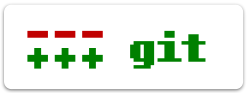
\includegraphics[height=35pt,keepaspectratio=true]{diagrames/git.png}
\end{tabular}
\end{center}
}